% !Mode:: "TeX:UTF-8"
\chapter{其他内容}
\label{chap:others}

\section{如何获得eps格式}
在文档中插入一张图片首先需要将图片转换为eps格式才能正确的显示,在这里推荐使用Adobe Acrobat Pro来进行转换。首先,假定你有了一张*.jpg格式或者*.png格式等的图片,正确安装Adobe Acrobat Pro后,在图片右键选择转换为转换为Adobe PDF,转换完后使用文件另存为命令进行保存,保存类型选择内嵌式PostScript(*.eps),点击下方的设置按钮按照图\ref{fig:fig2}进行设置即可,最后要删除掉figures文件夹下除eps以外的其他格式文件就可以在文档中显示图片了。
\begin{figure}[htbp]
\centering
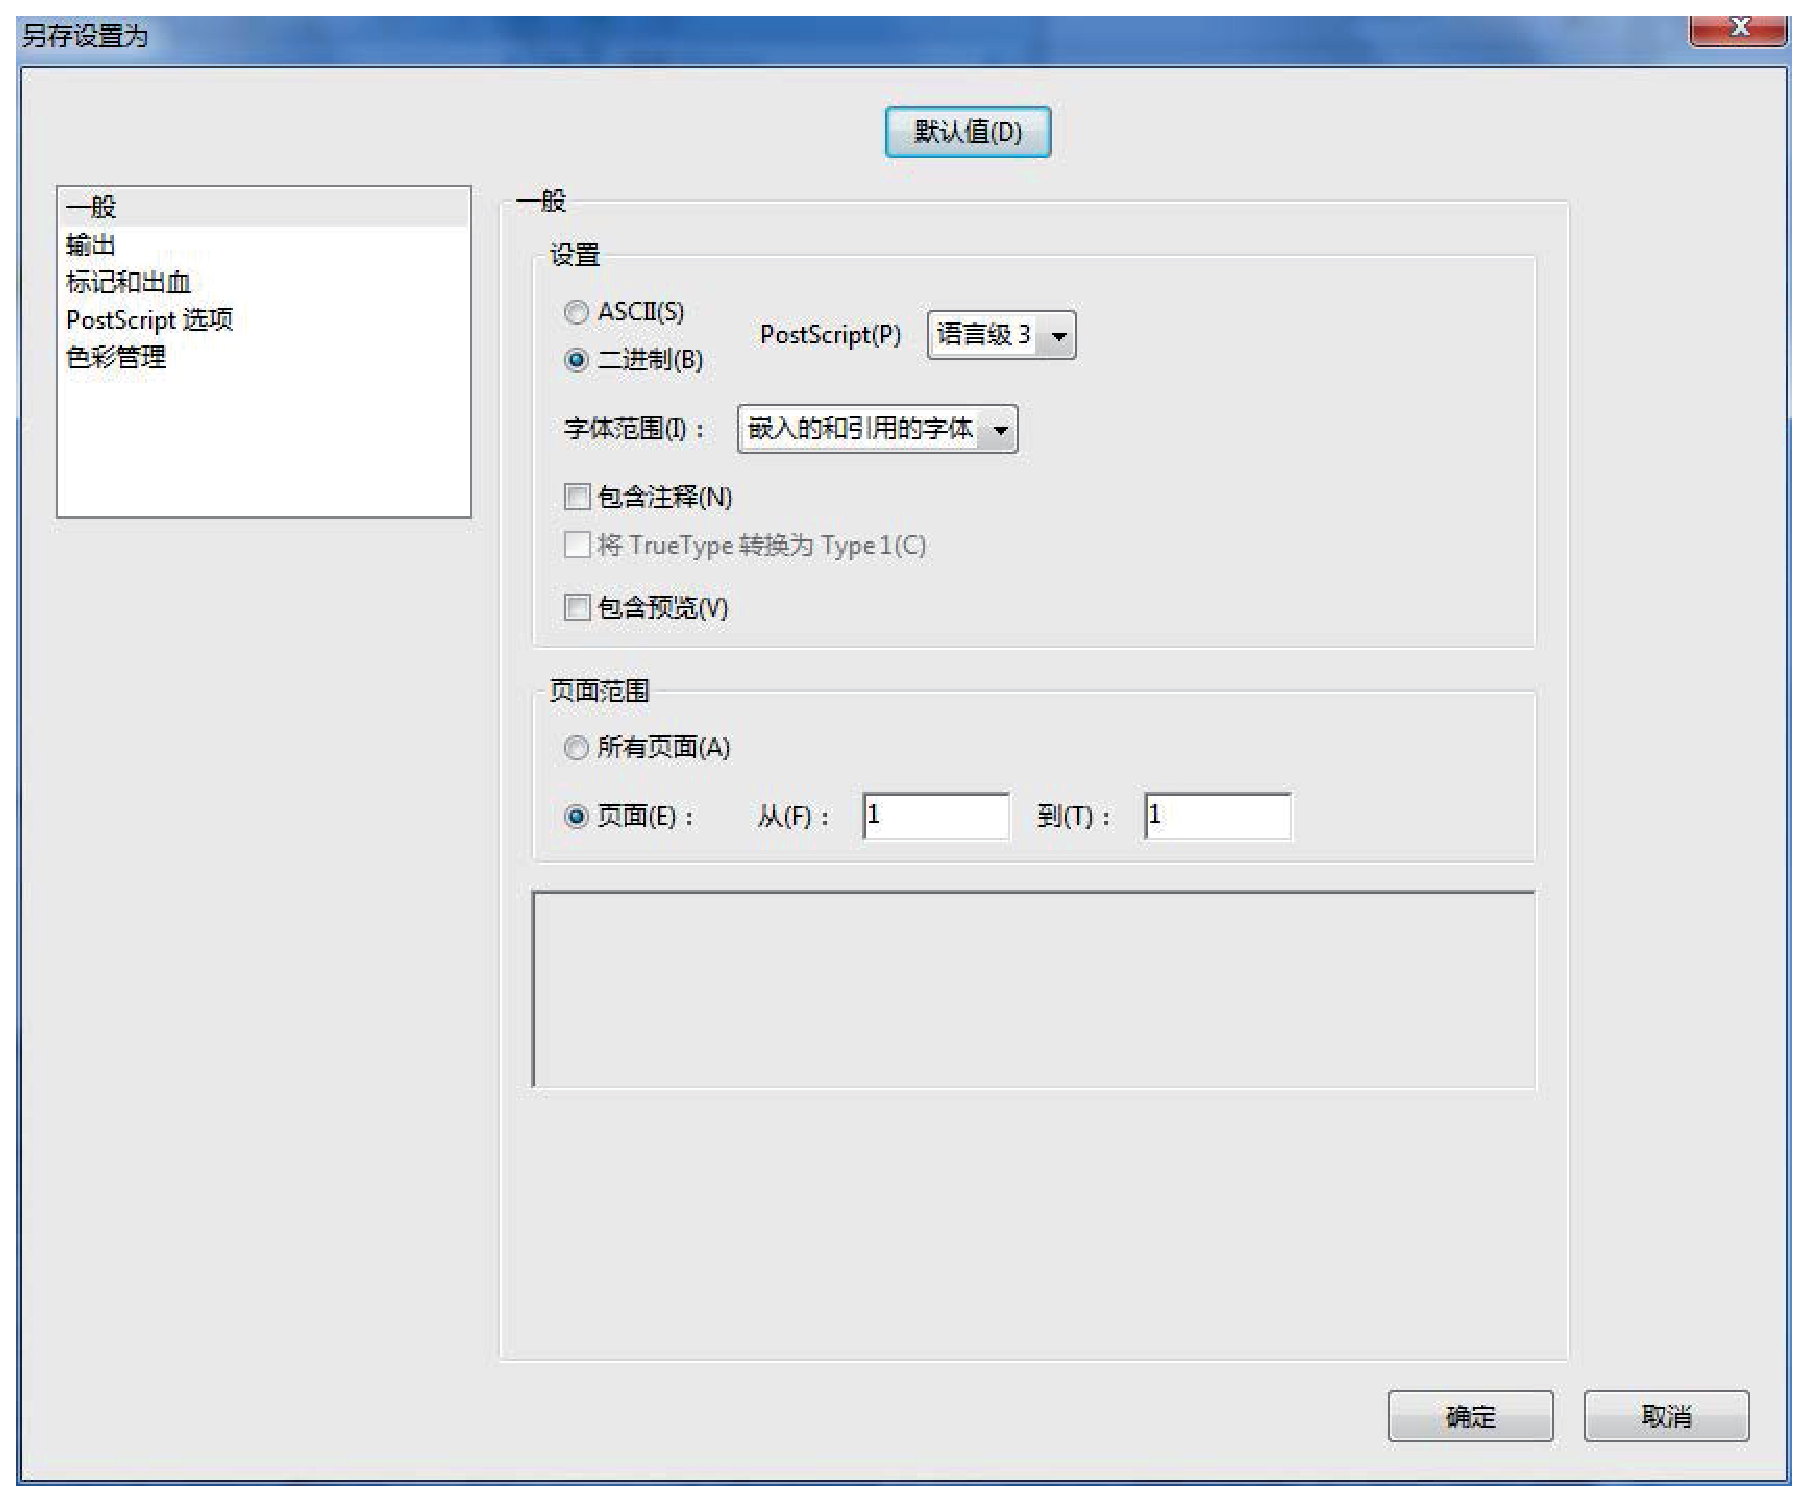
\includegraphics[width=\textwidth]{figures/piccvt}
\caption{设置示意图}\label{fig:fig2}
\vspace{\baselineskip}
\end{figure}
\section{如何引用参考文献}
由于一些原因,目前中国大陆无法使用Google Scholar,但是还好我们还有bing学术,bing学术同样有兼容BibTeX 的
参考文献信息。使用时也相当简单,如图\ref{fig:subfig2}所示,只要先搜到你想要引用的论文,然后在图\ref{fig:subfig2}-a中点击下方的引用出现图b,选择BibTeX即可出现引用信息如图\ref{fig:fig3},将这几行文字复制到references文件夹下的reference.bib文件里就可以在文档中进行引用了,当然有时也需要少量修改才行,引用时使用命令$\backslash$cite\{引用信息第一行的内容(必须是英文)\},如$\backslash$cite\{zhu2015a\}\cite{zhu2015a}。
\begin{figure}[htbp]
  \centering
  \subfigure[搜索结果]{
            \label{fig:subfig2:subsubfig1}
            
\includegraphics[width=0.4\textwidth]{figures/search}}
  \subfigure[引用信息]{
            \label{fig:subfig2:subsubfig2}
            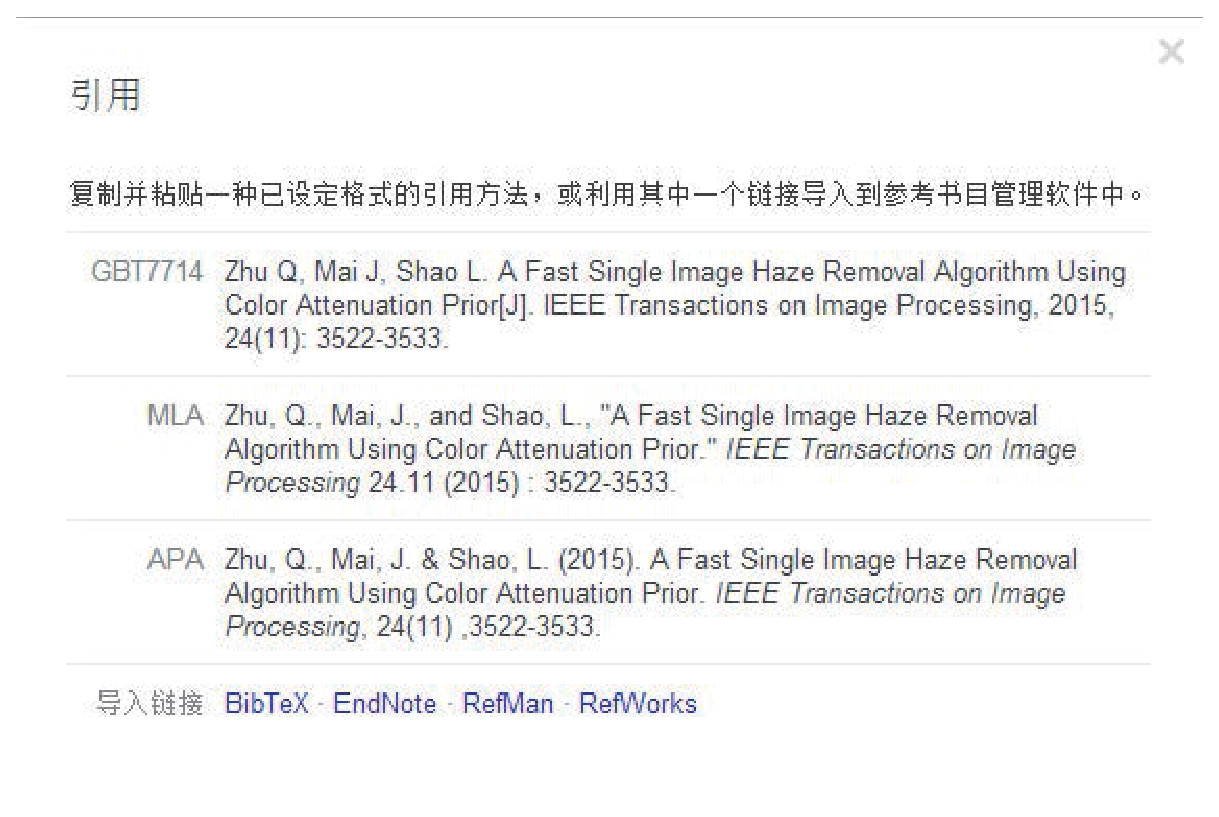
\includegraphics[width=0.4\textwidth]{figures/refers}}
  \caption{获取参考文献信息}\label{fig:subfig2}
\end{figure}

\begin{figure}[htbp]
  	\centering
  	
\includegraphics[width=0.8\textwidth]{figures/refresult}
  	\caption{待修改的引用信息}\label{fig:fig3}
\end{figure}

\section{使用算法环境}
控制学院的同学做毕业设计不少遇到写代码的情况,在论文中阐述自己的算法实现也是常有的事,一些宏包也专门给我们提供了一个专门用来放置伪代码片段的一个环境。\href{http://blog.sina.com.cn/s/blog_5e16f1770100lp7u.html}{示例}如下:\\
\begin{algorithm}[H]
\caption{identifyRowContext}
\KwIn{$r_i$ , $Backgrd(T_i)$=${T_1,T_2,\ldots,T_n}$ and similarity threshold $\theta_r$}
\KwOut{$con(r_i)$}
$con(r_i)= \Phi$\;
\For{$j=1;j \le n;j \ne i$}
{
 float $maxSim=0$\;
 $r^{maxSim}=null$\;
  \While{not end of $T_j$}
 {
     compute Jaro($r_i,r_m$)($r_m \in T_j$)\;
     \If{$(Jaro(r_i,r_m) \ge \theta _r) \wedge ((Jaro(r_i,r_m) \ge r^{maxSim}) $}
      {
           replace $r^maxSim$ with $r_m$\;
      }   
 }
$con(r_i)=con(r_i) \cup {r^{maxSim}}$\;
}
return $con(r_i)$\;
\end{algorithm}

%\begin{verbatim}\end{verbatim}
